% !TEX encoding = UTF-8 Unicode
\documentclass[10pt]{standalone}\usepackage{tikz}
\usepackage{fontspec}
\setmainfont{Arial}
\setsansfont{Arial}\begin{document}

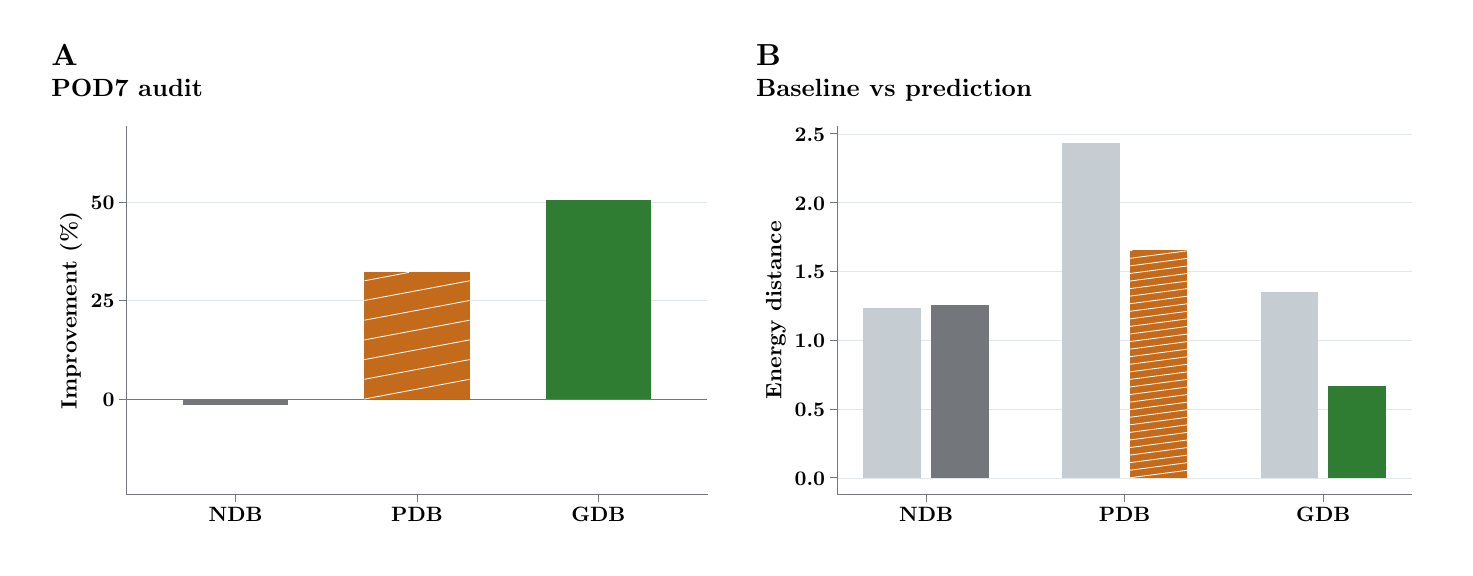
\begin{tikzpicture}[x=1pt,y=1pt]
\definecolor{fillColor}{RGB}{255,255,255}
\path[use as bounding box,fill=fillColor,fill opacity=0.00] (0,0) rectangle (512.15,187.79);
\begin{scope}
\path[clip] (  0.00,  0.00) rectangle (512.15,187.79);
\definecolor{drawColor}{RGB}{0,0,0}

\node[text=drawColor,anchor=base west,inner sep=0pt, outer sep=0pt, scale=  1.10] at (  8.54,174.22) {\bfseries A};

\node[text=drawColor,anchor=base west,inner sep=0pt, outer sep=0pt, scale=  0.90] at (  8.54,162.85) {\bfseries POD7 audit};
\end{scope}
\begin{scope}
\path[clip] (  8.54,  4.27) rectangle (248.96,157.34);
\definecolor{fillColor}{RGB}{255,255,255}

\path[fill=fillColor] (  8.54,  4.27) rectangle (248.96,157.34);
\end{scope}
\begin{scope}
\path[clip] ( 35.85, 19.07) rectangle (245.55,152.22);
\definecolor{fillColor}{RGB}{255,255,255}

\path[fill=fillColor] ( 35.85, 19.07) rectangle (245.55,152.22);
\definecolor{drawColor}{RGB}{226,231,235}

\path[draw=drawColor,line width= 0.2pt,line join=round] ( 35.85, 53.61) --
	(245.55, 53.61);

\path[draw=drawColor,line width= 0.2pt,line join=round] ( 35.85, 89.21) --
	(245.55, 89.21);

\path[draw=drawColor,line width= 0.2pt,line join=round] ( 35.85,124.81) --
	(245.55,124.81);
\definecolor{fillColor}{RGB}{115,119,123}

\path[fill=fillColor] ( 56.16, 51.49) rectangle ( 94.17, 53.61);
\definecolor{fillColor}{RGB}{196,106,27}

\path[fill=fillColor] (121.69, 53.61) rectangle (159.70, 99.35);
\definecolor{fillColor}{RGB}{46,125,50}

\path[fill=fillColor] (187.22, 53.61) rectangle (225.23,125.69);
\definecolor{drawColor}{RGB}{115,119,123}

\path[draw=drawColor,line width= 0.3pt,line join=round] ( 35.85, 53.61) -- (245.55, 53.61);
\definecolor{drawColor}{RGB}{255,255,255}

\path[draw=drawColor,line width= 0.3pt,line join=round] (121.69, 53.61) -- (159.70, 60.73);

\path[draw=drawColor,line width= 0.3pt,line join=round] (121.69, 60.73) -- (159.70, 67.85);

\path[draw=drawColor,line width= 0.3pt,line join=round] (121.69, 67.85) -- (159.70, 74.97);

\path[draw=drawColor,line width= 0.3pt,line join=round] (121.69, 74.97) -- (159.70, 82.09);

\path[draw=drawColor,line width= 0.3pt,line join=round] (121.69, 82.09) -- (159.70, 89.21);

\path[draw=drawColor,line width= 0.3pt,line join=round] (121.69, 89.21) -- (159.70, 96.33);

\path[draw=drawColor,line width= 0.3pt,line join=round] (121.69, 96.33) -- (137.80, 99.35);
\end{scope}
\begin{scope}
\path[clip] (  0.00,  0.00) rectangle (512.15,187.79);
\definecolor{drawColor}{RGB}{115,119,123}

\path[draw=drawColor,line width= 0.3pt,line join=round,line cap=rect] ( 35.85, 19.07) --
	( 35.85,152.22);
\end{scope}
\begin{scope}
\path[clip] (  0.00,  0.00) rectangle (512.15,187.79);
\definecolor{drawColor}{RGB}{0,0,0}

\node[text=drawColor,anchor=base east,inner sep=0pt, outer sep=0pt, scale=  0.75] at ( 31.40, 50.92) {\bfseries 0};

\node[text=drawColor,anchor=base east,inner sep=0pt, outer sep=0pt, scale=  0.75] at ( 31.40, 86.52) {\bfseries 25};

\node[text=drawColor,anchor=base east,inner sep=0pt, outer sep=0pt, scale=  0.75] at ( 31.40,122.13) {\bfseries 50};
\end{scope}
\begin{scope}
\path[clip] (  0.00,  0.00) rectangle (512.15,187.79);
\definecolor{drawColor}{RGB}{115,119,123}

\path[draw=drawColor,line width= 0.3pt,line join=round] ( 33.00, 53.61) --
	( 35.85, 53.61);

\path[draw=drawColor,line width= 0.3pt,line join=round] ( 33.00, 89.21) --
	( 35.85, 89.21);

\path[draw=drawColor,line width= 0.3pt,line join=round] ( 33.00,124.81) --
	( 35.85,124.81);
\end{scope}
\begin{scope}
\path[clip] (  0.00,  0.00) rectangle (512.15,187.79);
\definecolor{drawColor}{RGB}{115,119,123}

\path[draw=drawColor,line width= 0.3pt,line join=round,line cap=rect] ( 35.85, 19.07) --
	(245.55, 19.07);
\end{scope}
\begin{scope}
\path[clip] (  0.00,  0.00) rectangle (512.15,187.79);
\definecolor{drawColor}{RGB}{115,119,123}

\path[draw=drawColor,line width= 0.3pt,line join=round] ( 75.17, 16.23) --
	( 75.17, 19.07);

\path[draw=drawColor,line width= 0.3pt,line join=round] (140.70, 16.23) --
	(140.70, 19.07);

\path[draw=drawColor,line width= 0.3pt,line join=round] (206.23, 16.23) --
	(206.23, 19.07);
\end{scope}
\begin{scope}
\path[clip] (  0.00,  0.00) rectangle (512.15,187.79);
\definecolor{drawColor}{RGB}{0,0,0}

\node[text=drawColor,anchor=base,inner sep=0pt, outer sep=0pt, scale=  0.75] at ( 75.17,  9.26) {\bfseries NDB};

\node[text=drawColor,anchor=base,inner sep=0pt, outer sep=0pt, scale=  0.75] at (140.70,  9.26) {\bfseries PDB};

\node[text=drawColor,anchor=base,inner sep=0pt, outer sep=0pt, scale=  0.75] at (206.23,  9.26) {\bfseries GDB};
\end{scope}
\begin{scope}
\path[clip] (  0.00,  0.00) rectangle (512.15,187.79);
\definecolor{drawColor}{RGB}{0,0,0}

\node[text=drawColor,rotate= 90.00,anchor=base,inner sep=0pt, outer sep=0pt, scale=  0.80] at ( 17.68, 85.65) {\bfseries Improvement ({\%})};
\end{scope}
\begin{scope}
\path[clip] (  0.00,  0.00) rectangle (512.15,187.79);
\definecolor{drawColor}{RGB}{0,0,0}

\node[text=drawColor,anchor=base west,inner sep=0pt, outer sep=0pt, scale=  1.10] at (263.19,174.22) {\bfseries B};

\node[text=drawColor,anchor=base west,inner sep=0pt, outer sep=0pt, scale=  0.90] at (263.19,162.85) {\bfseries Baseline vs prediction};
\end{scope}
\begin{scope}
\path[clip] (263.19,  4.27) rectangle (503.61,157.34);
\definecolor{fillColor}{RGB}{255,255,255}

\path[fill=fillColor] (263.19,  4.27) rectangle (503.61,157.34);
\end{scope}
\begin{scope}
\path[clip] (292.58, 19.07) rectangle (500.20,152.22);
\definecolor{fillColor}{RGB}{255,255,255}

\path[fill=fillColor] (292.58, 19.07) rectangle (500.20,152.22);
\definecolor{drawColor}{RGB}{226,231,235}

\path[draw=drawColor,line width= 0.2pt,line join=round] (292.58, 25.13) --
	(500.20, 25.13);

\path[draw=drawColor,line width= 0.2pt,line join=round] (292.58, 49.99) --
	(500.20, 49.99);

\path[draw=drawColor,line width= 0.2pt,line join=round] (292.58, 74.85) --
	(500.20, 74.85);

\path[draw=drawColor,line width= 0.2pt,line join=round] (292.58, 99.71) --
	(500.20, 99.71);

\path[draw=drawColor,line width= 0.2pt,line join=round] (292.58,124.56) --
	(500.20,124.56);

\path[draw=drawColor,line width= 0.2pt,line join=round] (292.58,149.42) --
	(500.20,149.42);
\definecolor{fillColor}{RGB}{197,204,210}

\path[fill=fillColor] (302.02, 25.13) rectangle (322.83, 86.49);

\path[fill=fillColor] (373.78, 25.13) rectangle (394.60,146.17);

\path[fill=fillColor] (445.55, 25.13) rectangle (466.36, 92.41);
\definecolor{fillColor}{RGB}{115,119,123}

\path[fill=fillColor] (326.42, 25.13) rectangle (347.23, 87.40);
\definecolor{fillColor}{RGB}{196,106,27}

\path[fill=fillColor] (398.19, 25.13) rectangle (419.00,107.29);
\definecolor{fillColor}{RGB}{46,125,50}

\path[fill=fillColor] (469.95, 25.13) rectangle (490.76, 58.35);
\definecolor{drawColor}{RGB}{255,255,255}

\path[draw=drawColor,line width= 0.3pt,line join=round] (398.19, 25.13) -- (419.00, 27.86);

\path[draw=drawColor,line width= 0.3pt,line join=round] (398.19, 27.86) -- (419.00, 30.60);

\path[draw=drawColor,line width= 0.3pt,line join=round] (398.19, 30.60) -- (419.00, 33.33);

\path[draw=drawColor,line width= 0.3pt,line join=round] (398.19, 33.33) -- (419.00, 36.06);

\path[draw=drawColor,line width= 0.3pt,line join=round] (398.19, 36.06) -- (419.00, 38.80);

\path[draw=drawColor,line width= 0.3pt,line join=round] (398.19, 38.80) -- (419.00, 41.53);

\path[draw=drawColor,line width= 0.3pt,line join=round] (398.19, 41.53) -- (419.00, 44.27);

\path[draw=drawColor,line width= 0.3pt,line join=round] (398.19, 44.27) -- (419.00, 47.00);

\path[draw=drawColor,line width= 0.3pt,line join=round] (398.19, 47.00) -- (419.00, 49.74);

\path[draw=drawColor,line width= 0.3pt,line join=round] (398.19, 49.74) -- (419.00, 52.47);

\path[draw=drawColor,line width= 0.3pt,line join=round] (398.19, 52.47) -- (419.00, 55.21);

\path[draw=drawColor,line width= 0.3pt,line join=round] (398.19, 55.21) -- (419.00, 57.94);

\path[draw=drawColor,line width= 0.3pt,line join=round] (398.19, 57.94) -- (419.00, 60.68);

\path[draw=drawColor,line width= 0.3pt,line join=round] (398.19, 60.68) -- (419.00, 63.41);

\path[draw=drawColor,line width= 0.3pt,line join=round] (398.19, 63.41) -- (419.00, 66.14);

\path[draw=drawColor,line width= 0.3pt,line join=round] (398.19, 66.14) -- (419.00, 68.88);

\path[draw=drawColor,line width= 0.3pt,line join=round] (398.19, 68.88) -- (419.00, 71.61);

\path[draw=drawColor,line width= 0.3pt,line join=round] (398.19, 71.61) -- (419.00, 74.35);

\path[draw=drawColor,line width= 0.3pt,line join=round] (398.19, 74.35) -- (419.00, 77.08);

\path[draw=drawColor,line width= 0.3pt,line join=round] (398.19, 77.08) -- (419.00, 79.82);

\path[draw=drawColor,line width= 0.3pt,line join=round] (398.19, 79.82) -- (419.00, 82.55);

\path[draw=drawColor,line width= 0.3pt,line join=round] (398.19, 82.55) -- (419.00, 85.29);

\path[draw=drawColor,line width= 0.3pt,line join=round] (398.19, 85.29) -- (419.00, 88.02);

\path[draw=drawColor,line width= 0.3pt,line join=round] (398.19, 88.02) -- (419.00, 90.76);

\path[draw=drawColor,line width= 0.3pt,line join=round] (398.19, 90.76) -- (419.00, 93.49);

\path[draw=drawColor,line width= 0.3pt,line join=round] (398.19, 93.49) -- (419.00, 96.22);

\path[draw=drawColor,line width= 0.3pt,line join=round] (398.19, 96.22) -- (419.00, 98.96);

\path[draw=drawColor,line width= 0.3pt,line join=round] (398.19, 98.96) -- (419.00,101.69);

\path[draw=drawColor,line width= 0.3pt,line join=round] (398.19,101.69) -- (419.00,104.43);

\path[draw=drawColor,line width= 0.3pt,line join=round] (398.19,104.43) -- (419.00,107.16);

\path[draw=drawColor,line width= 0.3pt,line join=round] (398.19,107.16) -- (399.16,107.29);
\end{scope}
\begin{scope}
\path[clip] (  0.00,  0.00) rectangle (512.15,187.79);
\definecolor{drawColor}{RGB}{115,119,123}

\path[draw=drawColor,line width= 0.3pt,line join=round,line cap=rect] (292.58, 19.07) --
	(292.58,152.22);
\end{scope}
\begin{scope}
\path[clip] (  0.00,  0.00) rectangle (512.15,187.79);
\definecolor{drawColor}{RGB}{0,0,0}

\node[text=drawColor,anchor=base east,inner sep=0pt, outer sep=0pt, scale=  0.75] at (288.14, 22.44) {\bfseries 0.0};

\node[text=drawColor,anchor=base east,inner sep=0pt, outer sep=0pt, scale=  0.75] at (288.14, 47.30) {\bfseries 0.5};

\node[text=drawColor,anchor=base east,inner sep=0pt, outer sep=0pt, scale=  0.75] at (288.14, 72.16) {\bfseries 1.0};

\node[text=drawColor,anchor=base east,inner sep=0pt, outer sep=0pt, scale=  0.75] at (288.14, 97.02) {\bfseries 1.5};

\node[text=drawColor,anchor=base east,inner sep=0pt, outer sep=0pt, scale=  0.75] at (288.14,121.88) {\bfseries 2.0};

\node[text=drawColor,anchor=base east,inner sep=0pt, outer sep=0pt, scale=  0.75] at (288.14,146.74) {\bfseries 2.5};
\end{scope}
\begin{scope}
\path[clip] (  0.00,  0.00) rectangle (512.15,187.79);
\definecolor{drawColor}{RGB}{115,119,123}

\path[draw=drawColor,line width= 0.3pt,line join=round] (289.74, 25.13) --
	(292.58, 25.13);

\path[draw=drawColor,line width= 0.3pt,line join=round] (289.74, 49.99) --
	(292.58, 49.99);

\path[draw=drawColor,line width= 0.3pt,line join=round] (289.74, 74.85) --
	(292.58, 74.85);

\path[draw=drawColor,line width= 0.3pt,line join=round] (289.74, 99.71) --
	(292.58, 99.71);

\path[draw=drawColor,line width= 0.3pt,line join=round] (289.74,124.56) --
	(292.58,124.56);

\path[draw=drawColor,line width= 0.3pt,line join=round] (289.74,149.42) --
	(292.58,149.42);
\end{scope}
\begin{scope}
\path[clip] (  0.00,  0.00) rectangle (512.15,187.79);
\definecolor{drawColor}{RGB}{115,119,123}

\path[draw=drawColor,line width= 0.3pt,line join=round,line cap=rect] (292.58, 19.07) --
	(500.20, 19.07);
\end{scope}
\begin{scope}
\path[clip] (  0.00,  0.00) rectangle (512.15,187.79);
\definecolor{drawColor}{RGB}{115,119,123}

\path[draw=drawColor,line width= 0.3pt,line join=round] (324.63, 16.23) --
	(324.63, 19.07);

\path[draw=drawColor,line width= 0.3pt,line join=round] (396.39, 16.23) --
	(396.39, 19.07);

\path[draw=drawColor,line width= 0.3pt,line join=round] (468.16, 16.23) --
	(468.16, 19.07);
\end{scope}
\begin{scope}
\path[clip] (  0.00,  0.00) rectangle (512.15,187.79);
\definecolor{drawColor}{RGB}{0,0,0}

\node[text=drawColor,anchor=base,inner sep=0pt, outer sep=0pt, scale=  0.75] at (324.63,  9.26) {\bfseries NDB};

\node[text=drawColor,anchor=base,inner sep=0pt, outer sep=0pt, scale=  0.75] at (396.39,  9.26) {\bfseries PDB};

\node[text=drawColor,anchor=base,inner sep=0pt, outer sep=0pt, scale=  0.75] at (468.16,  9.26) {\bfseries GDB};
\end{scope}
\begin{scope}
\path[clip] (  0.00,  0.00) rectangle (512.15,187.79);
\definecolor{drawColor}{RGB}{0,0,0}

\node[text=drawColor,rotate= 90.00,anchor=base,inner sep=0pt, outer sep=0pt, scale=  0.80] at (272.33, 85.65) {\bfseries Energy distance};
\end{scope}
\end{tikzpicture}

\end{document}
